%\begin{figure}[htbp]

  
%\begin{subfigure}{0.49\textwidth}
%    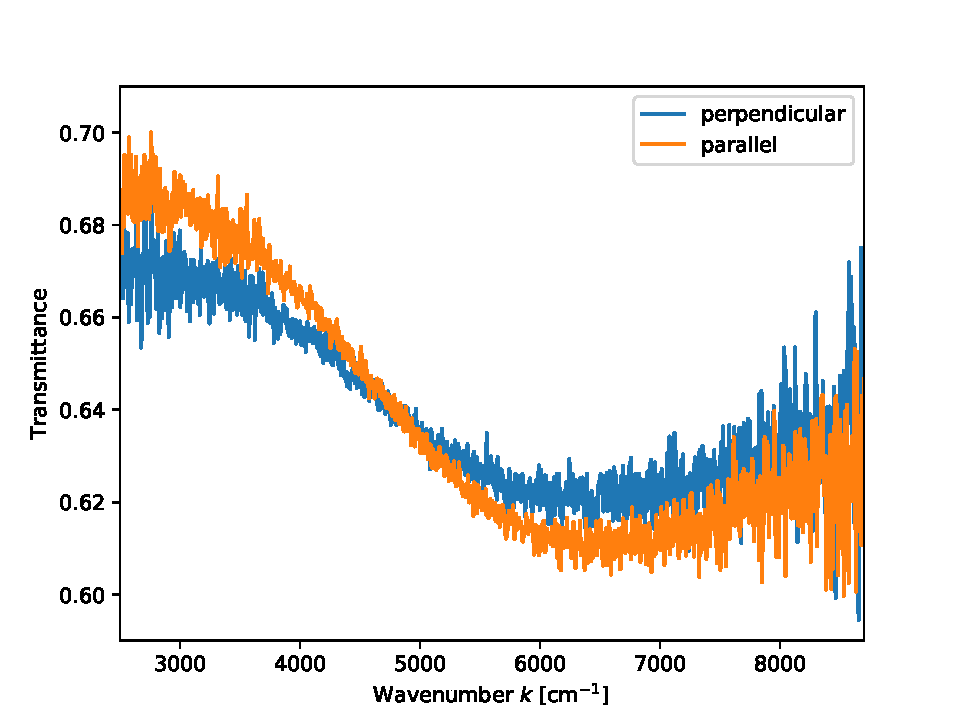
\includegraphics[width=\textwidth]{fullring.pdf}
%    \caption{fullrings  }
%    \label{fig:ftir_fr}
%\end{subfigure}
%\hfill
%\begin{subfigure}{0.49\textwidth}
%    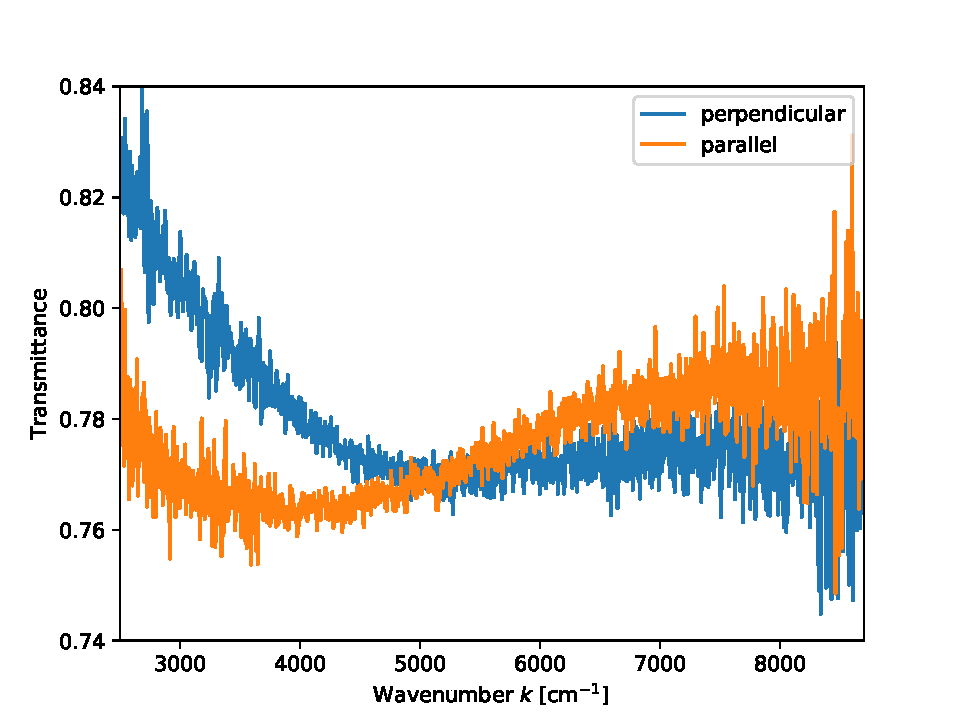
\includegraphics[width=\textwidth]{splitring.pdf}
%    \caption{splitrings}
%    \label{fig:ftir_sr}
%\end{subfigure}
%\caption{Transmittance spectra of fullrings (1) and splitrings (2) with a gap of $90^{\circ}$ between two different polarisations. }
%\label{fig:ftir}
  %\end{figure}

\begin{figure}
    \begin{subfigure}[t][18cm][b]{0.7\textwidth}
        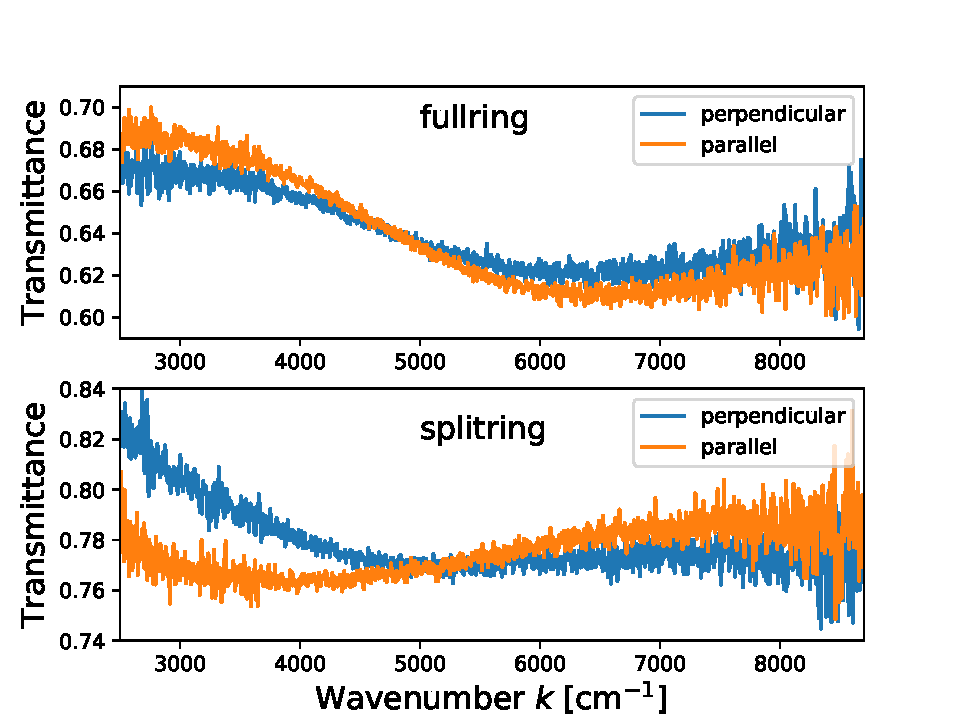
\includegraphics[scale=1.67]{FTIR.pdf}
    \end{subfigure}
    \begin{subfigure}[t][][b]{0.29\textwidth}
        \begin{tikzpicture}
            [x=0.6\textwidth, y=0.6\textwidth]
            \draw[fill=substrate] (0.5,0.5) rectangle (1.5,1.5);
            \draw[fill=gold]
                (1,1)++(55:.4)
                arc(55:-235:0.4)
                --($(1,1)+(-235:.25)$)
                arc(-235:55:.25)
                --($(1,1)+(55:.4)$);
            \draw[decoration={
                markings,
                mark=at position 0 with {\arrow[scale=4,shift={(0.008,0)},black]{<}};,
                mark=at position 1 with {\arrow[scale=4,black]{>}};
                },postaction={decorate}] (0.4,1.4)--(0.4,0.6);
            \draw[decoration={
                markings,
                mark=at position 0 with {\arrow[scale=4,shift={(0.008,0)},black]{<}};,
                mark=at position 1 with {\arrow[scale=4,black]{>}};
                },postaction={decorate}] (1.4,0.4)--(0.6,0.4);
            \draw
                (1,0.4) node[below] {parallel}
                (0.4,1) node[above,rotate=90] {perpendicular};
        \end{tikzpicture}
        \subcaption{Polarization}
    \end{subfigure}
    \caption{Reflectance spectra of fullrings  and splitrings  with a gap of $90^{\circ}$ between two different polarisations.}
\end{figure}

\begin{itemize}
 \item{Fourier-transform infrared spectroscopy (FTIR) is a technique to measure the transmission infrared spectra of a  solids, liquid or gas.} 
\item{There are different resonances visible in the reflectance spectra.}
\item{The difference for the SRRs between the two polarisations is too small in comparison to the theory. }
\item{The polarisation has an effect for the fullrings, which should't be the case. }
  \end{itemize}
